\documentclass[preprint,12pt,authoryear]{elsarticle}

\usepackage{amsmath}
\usepackage{graphicx}
\usepackage{booktabs}
\usepackage{tabularx}
\usepackage[T1]{fontenc}
\usepackage{lmodern}
\usepackage{textcomp}
\usepackage{lineno}
\usepackage[hidelinks]{hyperref}
\usepackage{xurl}

\newcommand{\kmsq}{km\textsuperscript{2}}
\newcommand{\cumecs}{m\textsuperscript{3}\,s\textsuperscript{-1}}
\newcommand{\Mcm}{million m\textsuperscript{3}}

\journal{Environmental Modelling \& Software}

\begin{document}

\begin{frontmatter}

\title{How far can one gauge mark and one radar image narrow parameter uncertainty in an open-data flood model? Sensitivity analysis of the 2018 Periyar flood}

\author[kahe]{Karthik V\corref{cor1}}
\ead{karthik.vasanthakumar@kahedu.edu.in}
\author[kahe]{Roopa D}
\cortext[cor1]{Corresponding author.}
\affiliation[kahe]{organization={Karpagam Academy of Higher Education},
            city={Coimbatore},
            state={Tamil Nadu},
            country={India}}

\begin{abstract}
Flood models of data-scarce tropical basins rest on global terrain, land-cover and water-mask data whose errors are rarely quantified together. We built an open-data two-dimensional D-Flow FM model of the lower Periyar River, Kerala, for the August 2018 flood using the HYDROLIB-core Python library, with boundary flows digitised from the Central Water Commission flood report. Validating the first model against the 12.4~m high-flood level (HFL) at Neeleswaram and a Sentinel-1 flood map exposed three structural errors (an inflow placed off the channel, a missing tidal outlet and an uncorrected surface model) and one missing input (the Chalakudy tributary). A Morris screening of the first model had not revealed them. On the final model, 180 Morris runs rank channel depth ($\mu^*$ = 149~\kmsq), floodplain roughness (101~\kmsq) and rating-curve error (65~\kmsq) first for peak flooded land, the same order as before the last revision; sea level is negligible (6~\kmsq). A 600-run Latin hypercube over the five leading factors was conditioned on the HFL (within 0.5~m) and on the radar map, used as a lower bound with an open-land hit-rate test. The 23 accepted runs give a peak flooded land of 146--198~\kmsq{} against a prior 5--95\% range of 107--329~\kmsq: a 77\% contraction of the range within the sampled ensemble (bootstrap 76--88\%), which falls to 49--72\% when the HFL tolerance is relaxed to 1~m. The HFL does most of the narrowing. Spatial agreement with the radar stays poor (critical success index at most 0.08 on all land), and none of eight structural variants, including a bare-earth terrain proxy and a 100~m grid, removes the excess flooding after the peak. The contraction is therefore conditional on the model structure, and is not a demonstrated reduction of predictive error.
\end{abstract}

\begin{highlights}
\item Open-data 2D model of the 2018 Periyar flood built and run with HYDROLIB-core
\item Validation exposed structural errors that sensitivity screening alone missed
\item Channel depth, floodplain roughness and rating error lead on the final model
\item One HFL mark and one radar scene narrow the flood-area range by about 77\%
\item The narrowing is conditional on model structure; radar spatial skill stays low
\end{highlights}

\begin{keyword}
global sensitivity analysis \sep Morris method \sep flood inundation modelling \sep D-Flow FM \sep Sentinel-1 \sep Kerala 2018 flood
\end{keyword}

\end{frontmatter}

\linenumbers

\section{Introduction}
\label{sec:intro}

The floods and landslides of August 2018 in Kerala took 433 lives \citep{pdna2018}. At Neeleswaram the Periyar peaked at about 8,800~\cumecs{} on 16 August and reached EL~12.4~m, 1.3~m above the previous record of 1974 \citep{cwc2018}. Events of this kind are increasingly modelled in two dimensions with open global data: the Copernicus DEM \citep{esa2021}, ESA WorldCover \citep{zanaga2022}, the JRC Global Surface Water record \citep{pekel2016} and global canopy-height maps \citep{tolan2024} make a 2D model possible almost anywhere. Each of these data sets carries errors, however. A digital surface model (DSM) is not a terrain model, and a coarse water mask misses channel geometry.

Global sensitivity analysis (GSA) is the standard way to find which of these uncertain inputs matter. Morris elementary effects \citep{morris1991}, summarised by the mean absolute effect $\mu^*$ \citep{campolongo2007}, screen many factors at low cost, within the broader framework of \citet{saltelli2008}. Conditioning on observations, as in GLUE \citep{beven1992}, then keeps only the parameter sets consistent with what was seen. Studies of 2D flood models usually assume a validated model and treat the observations separately. In data-scarce basins the model structure itself is uncertain, and few studies show how GSA and sparse observations interact, or report how validation changed the model before the GSA was run.

This paper makes four contributions:
\begin{enumerate}
\item A reproducible open-data workflow in Python (HYDROLIB-core) from global rasters to an ensemble of D-Flow FM runs, with every model version, run and score archived.
\item Evidence that validation against two cheap observations exposed structural errors that GSA alone did not, and a check that the factor ranking survives the last structural change.
\item A test of how far a single HFL mark and a single post-peak radar scene, under dense tree cover, can narrow the predicted flood area, with the narrowing quantified against ensemble size, acceptance rule, likelihood weighting and factor ranges.
\item Structural tests (terrain, channel mask, grid, tide) and a full contingency analysis against the radar map that bound what the parameter ensemble can claim.
\end{enumerate}

\subsection{Related work}

\paragraph{Uncertainty and sensitivity in flood inundation models}
\citet{teng2017} review the main classes of inundation model and how their uncertainty is analysed. \citet{pianosi2016} give a systematic review of sensitivity analysis for environmental models with a practical workflow; we follow its separation of factor screening (here Morris) from the conditioning of predictions. \citet{hall2005} applied variance-based (Sobol') sensitivity analysis to a raster inundation model of a River Thames reach checked against a radar flood outline, and found that channel roughness dominated the predicted outline and depth; splitting the channel into subreaches showed where the variance came from. \citet{pappenberger2005} carried uncertainty from ensemble rainfall forecasts through a rainfall-runoff model into LISFLOOD-FP, weighting ten roughness sets by their likelihood. \citet{savage2016} showed that grids coarser than about 50~m change flow paths and shift the best-fitting parameters, and that probabilistic flood maps lose reliability beyond about 100~m. This bears directly on our 200~m grid.

\paragraph{Conditioning on flood extent}
GLUE \citep{beven1992} rejects parameter sets that fail an observation and keeps the rest as behavioural. \citet{aronica2002} applied it to an inundation model using binary wet/dry pattern information, and \citet{bates2004} updated flood inundation likelihoods with flood extent data in a Bayesian scheme. \citet{montanari2009} used water stages derived from radar flood extents to calibrate and sequentially update a coupled hydrologic-hydraulic model. These studies use extents over largely open floodplains. In the lower Periyar most of the floodplain is under tree cover, so the radar extent can only bound the model from below, and we test what that weaker information can still constrain.

\paragraph{Terrain data}
Global elevation models such as the Copernicus DEM are surface models that include trees and buildings. \citet{hawker2022} produced FABDEM, a 30~m version of the Copernicus DEM with forests and buildings removed. We instead remove a fraction of canopy height and treat that fraction as an uncertain factor, so its effect on the flood can be measured rather than fixed in preprocessing, and we test a bare-earth proxy as a structural alternative.

\paragraph{The 2018 Kerala flood}
\citet{mishra2018} placed the August 2018 event in its hydroclimatic context. \citet{sudheer2019} modelled the Periyar basin with HEC-HMS and found that the Idukki peak release (about 1,860~\cumecs) was smaller than the flow of the nearly uncontrolled Perinjankutty tributary (about 3,500~\cumecs). Reservoir operation lowered the Neeleswaram peak by about 17\% compared with a no-dam case, and earlier emptying of the reservoirs would have lowered it by a further 16--21\%, still well above the bankfull capacity of about 4,200~\cumecs. They estimated a return period of about 142 years for the Neeleswaram flood. These studies are hydrological. We found no two-dimensional inundation model of the lower Periyar for 2018 whose uncertainty has been analysed.

\paragraph{What is new here}
Screening followed by behavioural selection is established practice, and we use standard methods (Morris, Latin hypercube, GLUE-style acceptance). The contribution is in how they are ordered and tested. First, the sparse observations are used to diagnose and revise the model structure before the GSA, and the screening is repeated on the final structure to show that the ranking is not an artefact of the revision. Second, a radar scene taken five days after the peak over a mostly forested floodplain is used as a lower bound with an open-land hit-rate test, and its limits are made explicit with a full contingency table. Third, the size of the resulting range contraction is treated as an uncertain quantity in its own right and reported against ensemble size, acceptance thresholds, likelihood weighting and factor ranges, rather than as a single figure. Fourth, structural variants show where the parameter ensemble stops being informative.

\section{Study area and data}
\label{sec:data}

The model covers the lower Periyar from near Neeleswaram (the CWC gauge-and-discharge site) to the Arabian Sea, from 76.15 to 76.55\textdegree E and 9.9 to 10.3\textdegree N (Fig.~\ref{fig:study}a). That includes the Munambam and Kochi inlets and the northern Vembanad backwater. The 2018 peak at Neeleswaram was about 8,800~\cumecs, with a high-flood level of EL~12.4~m \citep{cwc2018}. Table~\ref{tab:data} lists the data.

\begin{table}[htbp]
\centering
\caption{Data used to build and test the model.}
\label{tab:data}
\small
\begin{tabularx}{\textwidth}{@{}>{\raggedright\arraybackslash}X>{\raggedright\arraybackslash}X>{\raggedright\arraybackslash}p{2.8cm}l@{}}
\toprule
Data & Source & Use & Resolution \\
\midrule
Terrain (DSM) & Copernicus DEM GLO-30 \citep{esa2021} & Bed level & 30 m \\
Canopy height & Meta/WRI global canopy height \citep{tolan2024}; tiles averaged to the 200~m grid, values outside 0--100~m set to zero & DSM correction & 1 m \\
Land cover & ESA WorldCover 2021 \citep{zanaga2022} & Manning $n$ per class & 10 m \\
Permanent water & JRC Global Surface Water occurrence \citep{pekel2016} & Channel mask & 30 m \\
Neeleswaram discharge, 14--20 Aug & \citet{cwc2018}, Fig.~3 (digitised) & Upstream boundary & 6-hourly \\
Arangaly (Chalakudy) discharge, 14--17 Aug & \citet{cwc2018}, Fig.~13 (digitised) & Tributary inflow & digitised \\
Idukki spill, 9--18 Aug & \citet{cwc2018}, Fig.~4 (digitised) & Release factor & hourly \\
Idamalayar release, 1 Jul--23 Aug & \citet{cwc2018}, Fig.~5 (digitised) & Release factor & daily \\
HFL at Neeleswaram & \citet{cwc2018} & Validation & one value \\
Sentinel-1A GRD, 21 Aug 2018 00:40 UTC, and 28 Jul 2018 & Copernicus, AWS open data & Validation flood map & 20 m \\
\bottomrule
\end{tabularx}
\end{table}

The sea boundary uses a synthetic tide, $h(t) = 0.35\sin(2\pi t/12.42\,\mathrm{h}) + 0.20\sin(2\pi t/23.93\,\mathrm{h})$~m plus the sea-level offset factor, relative to the DEM datum (EGM2008), on the west and south edges, because no observed Kochi record could be reached. Its phase is arbitrary. The exact gauge coordinates are not published. The digitised series and their axis calibration are documented in the code archive.

\section{Methods}
\label{sec:methods}

\subsection{Hydrodynamic model}
D-Flow FM \citep{kernkamp2011} (computational kernel 1.2.184, built from the Deltares source code) runs on a 200~m rectilinear grid of 32,337 cells in UTM zone 43N, clipped to land below 20~m plus a 400~m corridor around the channel. The run spans 13 August 00:00 to 21 August 07:00 IST. The Copernicus DEM tiles are reprojected and aggregated to 200~m by averaging (and separately by minimum), the canopy height by averaging, the JRC water occurrence by maximum, so that any permanent water marks a cell as channel and narrow reaches stay connected, and WorldCover by mode. Every cell with water occurrence above 50\% is channel, with its bed set a channel depth below the lowest DSM value in the cell. Water cells not connected to the river are kept as channel cells; they exchange water with the floodplain only where they touch it. The floodplain bed is the mean DSM minus a canopy factor times the mean canopy height. Manning $n$ follows WorldCover classes (0.025--0.10). The upstream boundary takes the Neeleswaram discharge, which already includes the dam releases and the intervening catchment. A second inflow on the north edge carries the Chalakudy River, using the CWC Arangaly record (14--17 August), which then recedes in proportion to the Periyar. No local rainfall or other lateral inflow is included. Numerical settings: implicitness $\theta$ = 0.55, maximum Courant number 0.7, maximum time step 30~s (mean 28.7~s in the nominal run), wetting/drying threshold $10^{-4}$~m, bed level at faces from the mean of node values. The cumulative volume error of the nominal run is below 1~m\textsuperscript{3} against $6.9\times10^9$~m\textsuperscript{3} of boundary inflow. All model files are written with HYDROLIB-core.

\subsection{Uncertain factors}
Table~\ref{tab:factors} lists the eight factors and their ranges. All are sampled from independent uniform distributions. Three ranges rest on the size of known errors: the rating-curve error ($\pm$15\% on the whole Neeleswaram hydrograph, a common allowance for high-flow ratings), the two release multipliers ($\pm$20\%, for reporting and digitising error) and the sea-level offset (surge and datum uncertainty). The roughness multipliers span the usual spread of tabulated Manning values around the land-cover defaults. Channel depth and the canopy factor have no direct observation in this basin, so their ranges are chosen to explore model behaviour over all plausible values, and we read the conditioned values of these two factors with that in mind. The rating error and the release multipliers are not physically independent, because the Neeleswaram record already contains the releases; sampling them independently treats the release multipliers as an error in the timing and share of the released water on top of the gauge error.

\begin{table}[htbp]
\centering
\caption{Uncertain factors, their ranges (independent uniform sampling) and the basis of each range.}
\label{tab:factors}
\small
\begin{tabularx}{\textwidth}{@{}lp{2.4cm}>{\raggedright\arraybackslash}X>{\raggedright\arraybackslash}p{3.2cm}@{}}
\toprule
Factor & Range & Meaning & Basis \\
\midrule
n\_channel & 0.7--1.3 (--) & Multiplier on channel Manning $n$ & Tabulated spread \\
n\_floodplain & 0.6--1.5 (--) & Multiplier on floodplain Manning $n$ & Tabulated spread \\
channel\_depth & 2--8 m & Channel bed below the lowest DSM value in the cell & Exploratory (no bathymetry) \\
canopy\_factor & 0.3--0.9 (--) & Fraction of cell-mean canopy height subtracted from the DSM & Exploratory \\
q\_rating & 0.85--1.15 (--) & Multiplier on the whole Neeleswaram hydrograph & High-flow rating error \\
q\_idukki & 0.8--1.2 (--) & Scaled share of the Idukki spill, lagged 8 h & Reporting/digitising error \\
q\_idamalayar & 0.8--1.2 (--) & Scaled share of the Idamalayar release, lagged 4 h & Reporting/digitising error \\
tide\_offset & $-0.2$ to $+0.5$ m & Sea-level offset including surge & Surge and datum \\
\bottomrule
\end{tabularx}
\end{table}

\subsection{Screening}
A Morris design with 20 trajectories, 4 levels and the SALib default jump $\Delta = 2/3$ (180 runs, seed 42) was generated with SALib 1.6.0 \citep{herman2017}, and 95\% confidence intervals on $\mu^*$ come from 100 bootstrap resamples. $\mu^*$ measures the overall influence of a factor; a large $\sigma$ shows that the effect varies across the factor space, through non-linearity or interaction, without separating the two or giving the share of interaction. Each run is reduced to peak flooded land, peak flood volume, mean maximum depth, time to peak, the Neeleswaram peak level and the validation scores below. Cells that are wet at the start are excluded, so the metrics describe land that the flood inundated.

\subsection{Validation and conditioning}
\label{sec:validation}
\paragraph{HFL} The modelled level is the highest hourly median water level over the 10 channel cells within 500~m of the centre of the inflow section (76.49\textdegree E, 10.172--10.198\textdegree N), the reach where the Neeleswaram gauge lies, and it is compared with the HFL as a peak level. The CWC report gives the HFL as EL~12.4~m, which we take to be above mean sea level; we treat it as on the DEM datum, so any datum offset adds to the HFL uncertainty.

\paragraph{Radar} The Sentinel-1 flood map uses calibrated VV backscatter with a 5\,$\times$\,5 filter, below an Otsu threshold on the post-event scene ($-13.8$~dB) together with a drop of more than 3~dB from 28 July, aggregated to the 200~m grid as a flooded fraction. A cell counts as flooded above a fraction of 0.5, and permanent-water cells are excluded. C-band radar misses water under tree cover and in built-up land, so the radar's 22~\kmsq{} of open-water flooding is treated as a lower bound on the model's flooded land, not as a target.

\paragraph{Acceptance rule} A run is behavioural when its HFL error is within 0.5~m, its flooded land at the radar pass is at least 22~\kmsq, and it floods at least 75\% of the open-land cells (WorldCover cropland, grassland, bare and herbaceous wetland) that the radar shows as flooded. An earlier rule that also capped the model area at three times the radar's rejected every run of the final model (Section~\ref{sec:conditioning}).

\paragraph{Ensemble and what ``constrain'' means} The five leading factors were sampled by two Latin hypercubes, 200 runs (seed 42) and 400 runs (seed 43), with the other three at nominal values. By constraint we mean only the contraction of the predicted range of peak flooded land within the sampled ensemble, conditional on the model structure, the factor ranges and the acceptance rule. We do not claim that the accepted range is a calibrated predictive interval. The narrowing is $1 - w_\mathrm{post}/w_\mathrm{prior}$, where $w_\mathrm{post}$ is the full range of the accepted runs. Because the range of $n$ accepted runs covers on average $(n-1)/(n+1)$ of their distribution, $w_\mathrm{prior}$ is taken as the central interval of the prior ensemble with that coverage (like-for-like), and the prior 5--95\% interval is reported alongside. We test the narrowing in four ways: bootstrap resampling of the whole ensemble with the rule re-applied (5,000 resamples); a grid of HFL tolerances (0.25--1.5~m) and hit rates (0.5--0.9); an informal likelihood weighting in place of the yes/no rule, $L = \exp[-\tfrac12(e/s)^2]\,r^4$ for HFL error $e$, open-land hit rate $r$ and $s$ = 0.25, 0.5 or 1.0~m, with zero weight below 22~\kmsq; and removal of the lowest or highest fifth of each factor's range, as if the range had been set narrower.

\subsection{Structural tests}
Eight structural variants were rebuilt and run at nominal parameters: the nominal model; a bare-earth proxy that takes the lowest 30~m DSM pixel in each 200~m cell (FABDEM could not be downloaded from our computing environment); full canopy removal (factor 1.0); a wider channel mask (water occurrence above 25\%); 100~m and 400~m grids; and the tide scaled by 1.5 or shifted by half an M2 period (6.21~h). Each run is scored against the radar with the full contingency table: hits, misses, false alarms and correct negatives, hit rate, false-alarm ratio, critical success index (CSI), frequency bias and equitable threat score (ETS). The radar map was also rebuilt with the Otsu threshold moved by $\pm$1.5~dB and with change thresholds of 2 and 4~dB, and scored with a cell-fraction cut-off of 0.3 as well as 0.5.

\section{Results}
\label{sec:results}

\subsection{Validation changed the model before the GSA}
Four revisions brought the nominal model from a 10~m level error to about 2~m (Table~\ref{tab:versions}). Three corrected the model: the inflow moved onto the channel, the tidal outlet added, and the DSM corrected for canopy. One added a missing input, the Chalakudy River (v4), which doubled the share of radar-flooded land the model catches, from 28\% to 54\% (open land: 66\% to 91\%), because most radar flooding lies at the Chalakudy--Periyar confluence (Fig.~\ref{fig:study}). It also raised the total flooded land. A test with land infiltration of up to 10~mm\,h\textsuperscript{-1} removed only 25~\kmsq{} of it, so missing infiltration does not explain the excess.

\begin{table}[htbp]
\centering
\caption{Model revisions and their nominal scores against the two observations. Scores of different versions are not strictly comparable: v1 was scored at a different cell and v1--v2 at an earlier hour (footnote).}
\label{tab:versions}
\small
\begin{tabularx}{\textwidth}{@{}l>{\raggedright\arraybackslash}X>{\raggedleft\arraybackslash}p{2.2cm}>{\raggedleft\arraybackslash}p{3.2cm}@{}}
\toprule
Version & Change & HFL error (m) & Flooded land at radar pass (\kmsq) \\
\midrule
v1 & First open-data model & +10.4\textsuperscript{a} & 350 \\
v2 & Inflow on the channel, continuous channel, canopy correction & +2.3 & 149 \\
v3 & Kochi inlet and tidal south edge, run past the pass & +2.4 & 123 \\
v4 & Chalakudy River inflow added (CWC Arangaly record) & +2.4 & 190 \\
v5 & Chalakudy flow recedes after its record ends instead of holding 799~\cumecs & +2.4 & 180 \\
Radar & Sentinel-1, 21 Aug 2018 & 0 (HFL 12.4 m) & 22 (open water only) \\
\bottomrule
\end{tabularx}
\par\smallskip
\raggedright\footnotesize \textsuperscript{a}v1 was scored on the highest cell near the inflow, which sat 2~km off the mesh; later versions use channel cells. v1 and v2 are scored at hour 192, v3 to v5 at hour 198.
\end{table}

\begin{figure}[htbp]
\centering
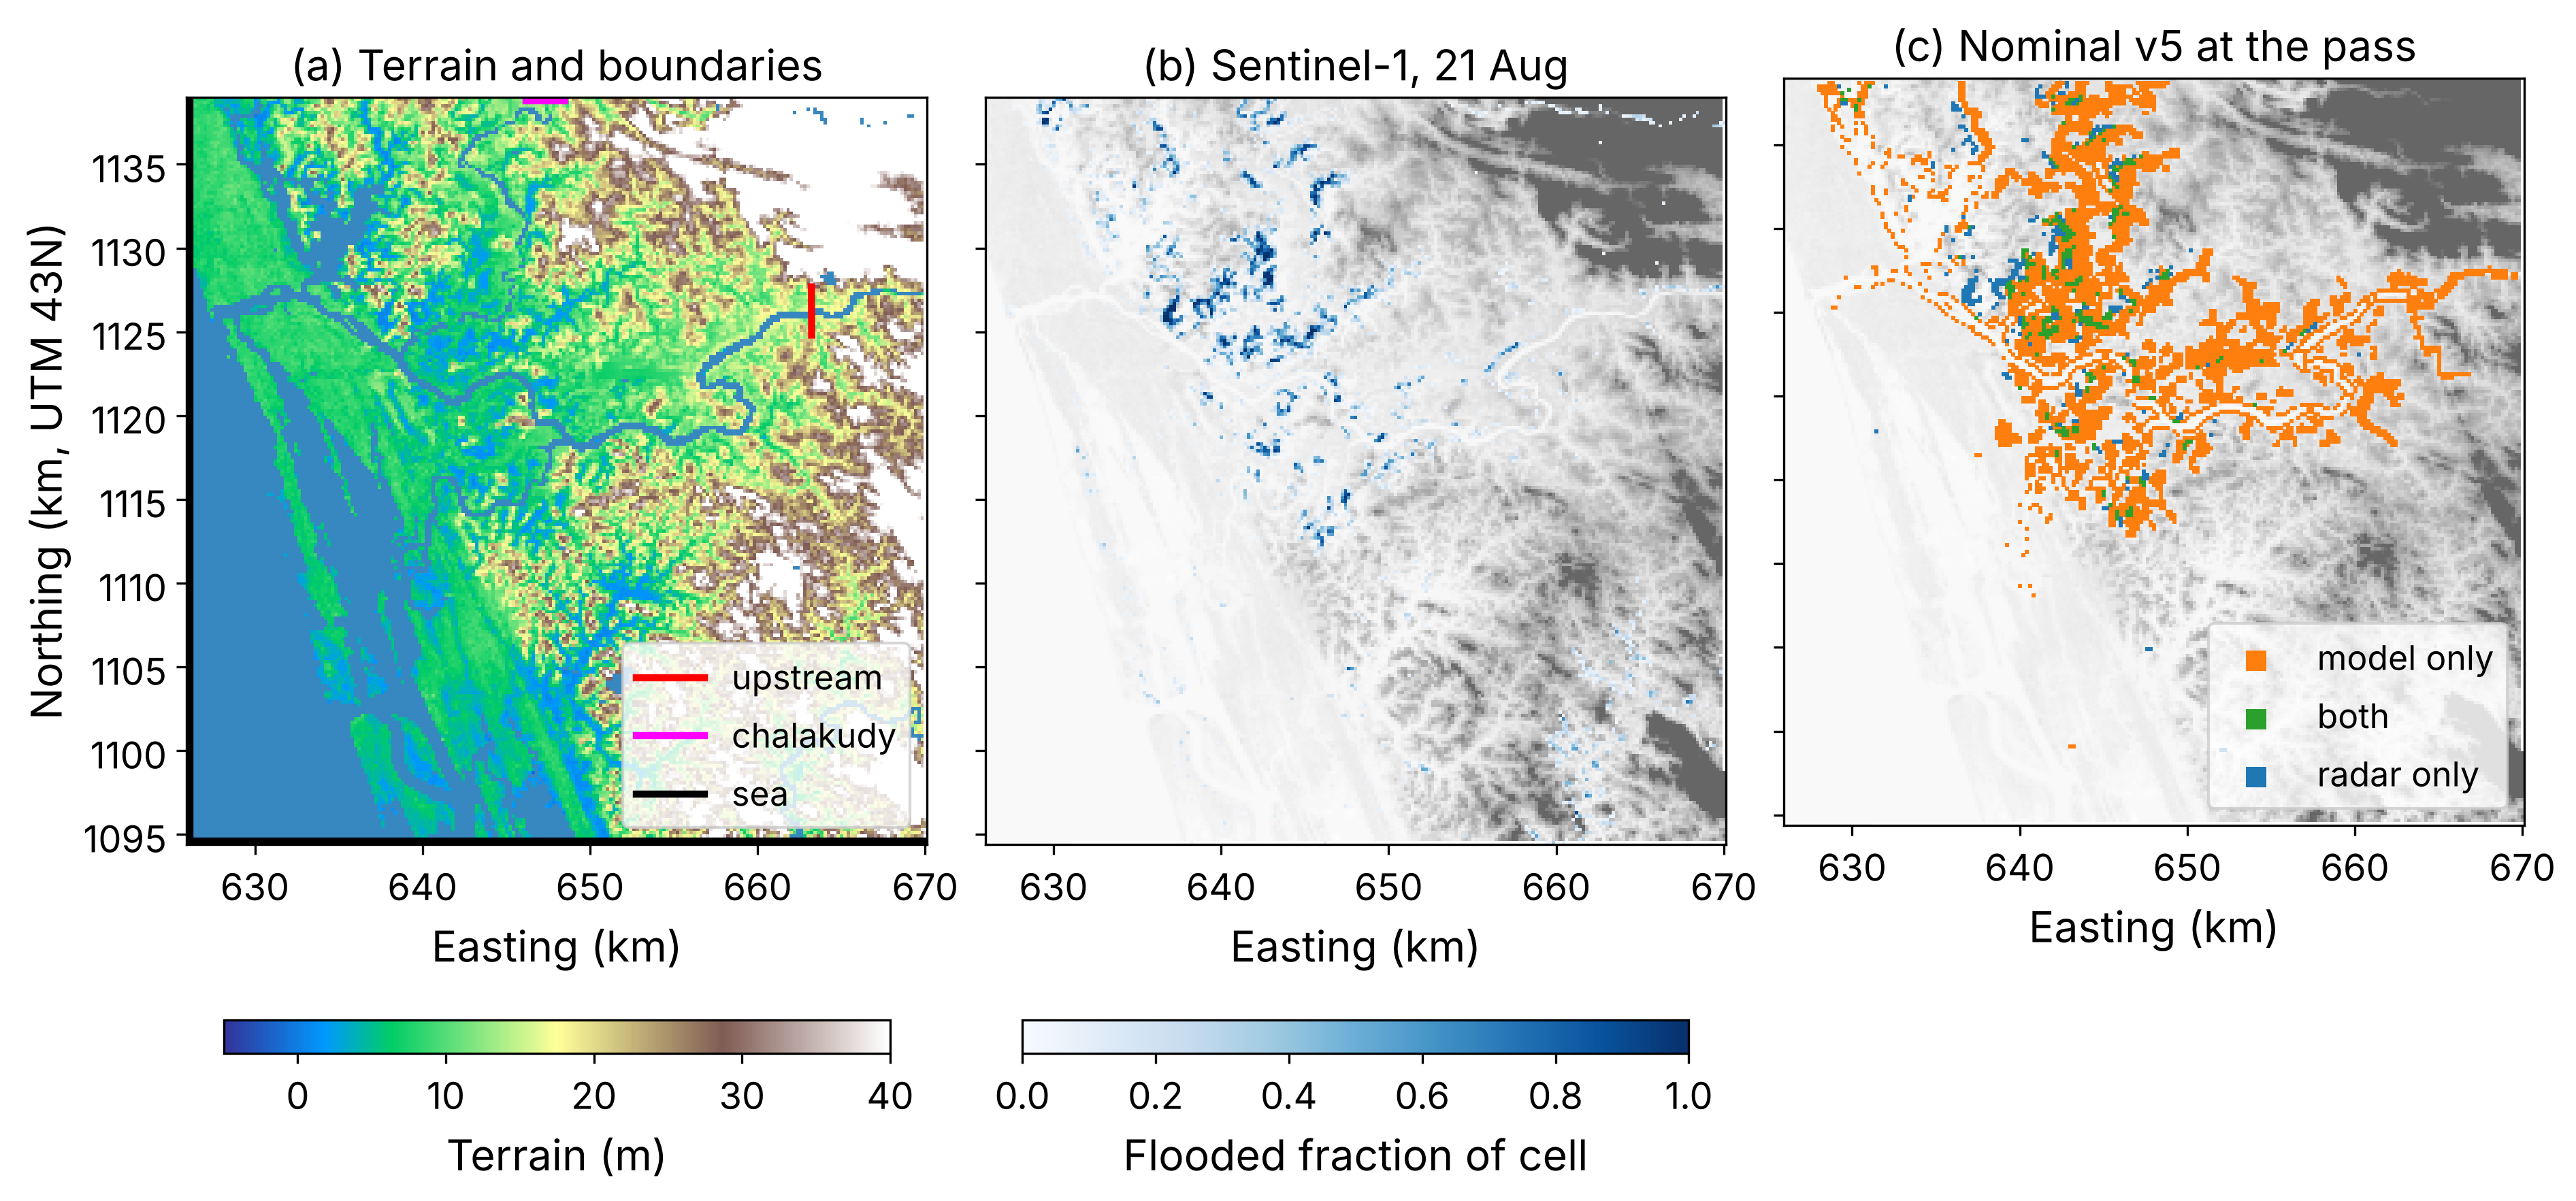
\includegraphics[width=\textwidth]{figures/fig1.png}
\caption{(a) Model terrain (canopy-corrected DSM), channel and boundaries. (b) Sentinel-1 open-water flood fraction, 21 August 2018 06:10 IST. (c) Nominal v5 model at the radar pass: flooded land in the model only, in both, and in the radar only.}
\label{fig:study}
\end{figure}

\subsection{Screening of the final model}
\label{sec:screening}
All 180 Morris runs on v5 completed. Peak flooded land ranged from 86 to 388~\kmsq{} and peak volume from 281 to 1,385~\Mcm. Channel depth, floodplain roughness and rating-curve error lead peak area, volume and the Neeleswaram level (Table~\ref{tab:morris}), and together account for 71\% of the summed $\mu^*$ for area. Floodplain roughness dominates timing ($\mu^*$ = 42~h for time to peak). Sea level is negligible inland of the inlets ($\mu^*$ = 6~\kmsq, and 0.00~m for the gauge level). High $\sigma$ for the top factors shows that their effects depend on the other factors. The three factors fixed in the conditioning ensemble (channel roughness, Idamalayar release and sea level) account for 11\% of the summed $\mu^*$ for area.

The same design on v4, before the change in the Chalakudy recession, gives the same order of all eight factors for peak area, peak volume, the gauge level and flooded land at the radar pass, with $\mu^*$ within 5\% for the leading three (v4: 150, 97 and 63~\kmsq). The gauge-level indices are identical, because the peak comes before the change. Only time to peak reorders: the canopy factor falls from second (23~h on v4) to fifth (10~h), and rating error rises to second (22~h); these shifts lie within the bootstrap confidence intervals. The five factors chosen for the conditioning ensemble are therefore still the five most influential for peak area on the final model. A first screening on v1 ranked the same top three factors, but on a model that failed both checks; it is reported only as a cautionary result.

\begin{table}[htbp]
\centering
\caption{Morris indices on the final model v5 (180 runs): $\mu^*$ with $\sigma$ in brackets, ordered by peak flooded land. The order for peak land, volume and level is the same on v4.}
\label{tab:morris}
\footnotesize
\begin{tabular}{@{}lrrrr@{}}
\toprule
Factor & Peak land & Peak volume & Time to peak & Peak level \\
 & (\kmsq) & (\Mcm) & (h) & (m) \\
\midrule
Channel depth & 149 (57) & 516 (271) & 12.5 (13.3) & 2.92 (0.63) \\
Floodplain roughness & 101 (96) & 414 (379) & 42.1 (52.0) & 2.86 (2.46) \\
Rating-curve error & 65 (73) & 258 (298) & 22.3 (38.4) & 2.00 (1.31) \\
Canopy factor & 41 (38) & 56 (118) & 10.4 (26.6) & 1.74 (1.98) \\
Idukki release & 38 (77) & 149 (309) & 18.9 (41.1) & 1.00 (1.78) \\
Channel roughness & 31 (16) & 119 (74) & 10.4 (20.8) & 1.00 (0.17) \\
Idamalayar release & 14 (38) & 56 (154) & 6.9 (11.2) & 0.36 (0.60) \\
Sea-level offset & 6 (1) & 5 (2) & 1.9 (4.1) & 0.00 (0.00) \\
\bottomrule
\end{tabular}
\end{table}

\subsection{Conditioning on observations}
\label{sec:conditioning}
All 600 Latin hypercube runs completed. 55 met the HFL within 0.5~m, 492 passed the radar test, and 23 passed both. The HFL test therefore does almost all of the narrowing (Fig.~\ref{fig:uncertainty}a); the radar test on its own removes only the runs that flood least. The prior peak flooded land spans 89--364~\kmsq{} (5--95\%: 107--329~\kmsq; median 220~\kmsq). The 23 accepted runs span 146--198~\kmsq{} (5--95\%: 152--182; median 166~\kmsq), and their peak volume 411--558~\Mcm{} against a prior 5--95\% range of 343--1,121~\Mcm. HFL residuals have a prior median of +1.9~m (5--95\%: $-1.45$ to $+3.58$~m); the accepted runs lie between $-0.28$ and $+0.49$~m (Fig.~\ref{fig:uncertainty}c).

The accepted range is 77\% narrower than the prior interval of equal expected coverage (92\%, 105--334~\kmsq) and 76\% narrower than the prior 5--95\% interval (Table~\ref{tab:robust}). Our first 200 runs alone gave 7 accepted runs, 158--182~\kmsq{} and 89\% narrowing; with three times as many runs the accepted range widened at both ends, mostly upward, and the narrowing settled at 76--77\%. The new 400 runs alone give 16 accepted runs, 146--198~\kmsq{} and 76\%, so the estimate is now stable to the sample. Bootstrap resampling gives 16--31 accepted runs and a narrowing of 76--88\% (5--95\%).

The narrowing depends on how strict the rule is (Fig.~\ref{fig:uncertainty}b). With the HFL within 0.5~m and hit rates of 0.70--0.85 it is 74--83\%; at $\pm$0.25~m it rises to 73--85\%; at $\pm$1.0~m, a tolerance comparable to the 0.9~m change in the gauge level between the 100~m and 200~m grids (Section~\ref{sec:structural}), it falls to 49--72\%. Replacing the yes/no rule by likelihood weights gives a weighted 5--95\% range of 136--181~\kmsq{} for $s$ = 0.25~m (52 effective runs; 79\% narrower), 136--219~\kmsq{} for $s$ = 0.5~m (121; 62\%) and 137--280~\kmsq{} for $s$ = 1.0~m (295; 35\%). Removing the lowest or highest fifth of any factor's range changes the narrowing to 73--79\%, except that dropping the highest canopy factors lowers the upper end of the accepted range to 171~\kmsq{} and raises it to 87\%.

\begin{table}[htbp]
\centering
\caption{Narrowing of the peak flooded-land range under different analysis choices (600-run ensemble unless stated).}
\label{tab:robust}
\small
\begin{tabularx}{\textwidth}{@{}>{\raggedright\arraybackslash}Xrrr@{}}
\toprule
Analysis & Accepted / effective runs & Range (\kmsq) & Narrowing \\
\midrule
First 200 runs, acceptance rule & 7 & 158--182 & 89\% \\
New 400 runs only, acceptance rule & 16 & 146--198 & 76\% \\
600 runs, acceptance rule (like-for-like) & 23 & 146--198 & 77\% \\
Bootstrap of 600 runs (5--95\%) & 16--31 & -- & 76--88\% \\
HFL $\pm$0.5~m, hit rate 0.70--0.85 & 3--47 & -- & 74--83\% \\
HFL $\pm$1.0~m, hit rate 0.50--0.85 & 26--131 & -- & 49--72\% \\
Likelihood weights, $s$ = 0.25~m & 52 & 136--181\textsuperscript{a} & 79\% \\
Likelihood weights, $s$ = 0.5~m & 121 & 136--219\textsuperscript{a} & 62\% \\
Likelihood weights, $s$ = 1.0~m & 295 & 137--280\textsuperscript{a} & 35\% \\
One factor range cut by a fifth (10 cases) & 10--22 & -- & 73--87\% \\
\bottomrule
\end{tabularx}
\par\smallskip
\raggedright\footnotesize \textsuperscript{a}Weighted 5--95\% range, compared with the prior 5--95\% range.
\end{table}

\begin{figure}[htbp]
\centering
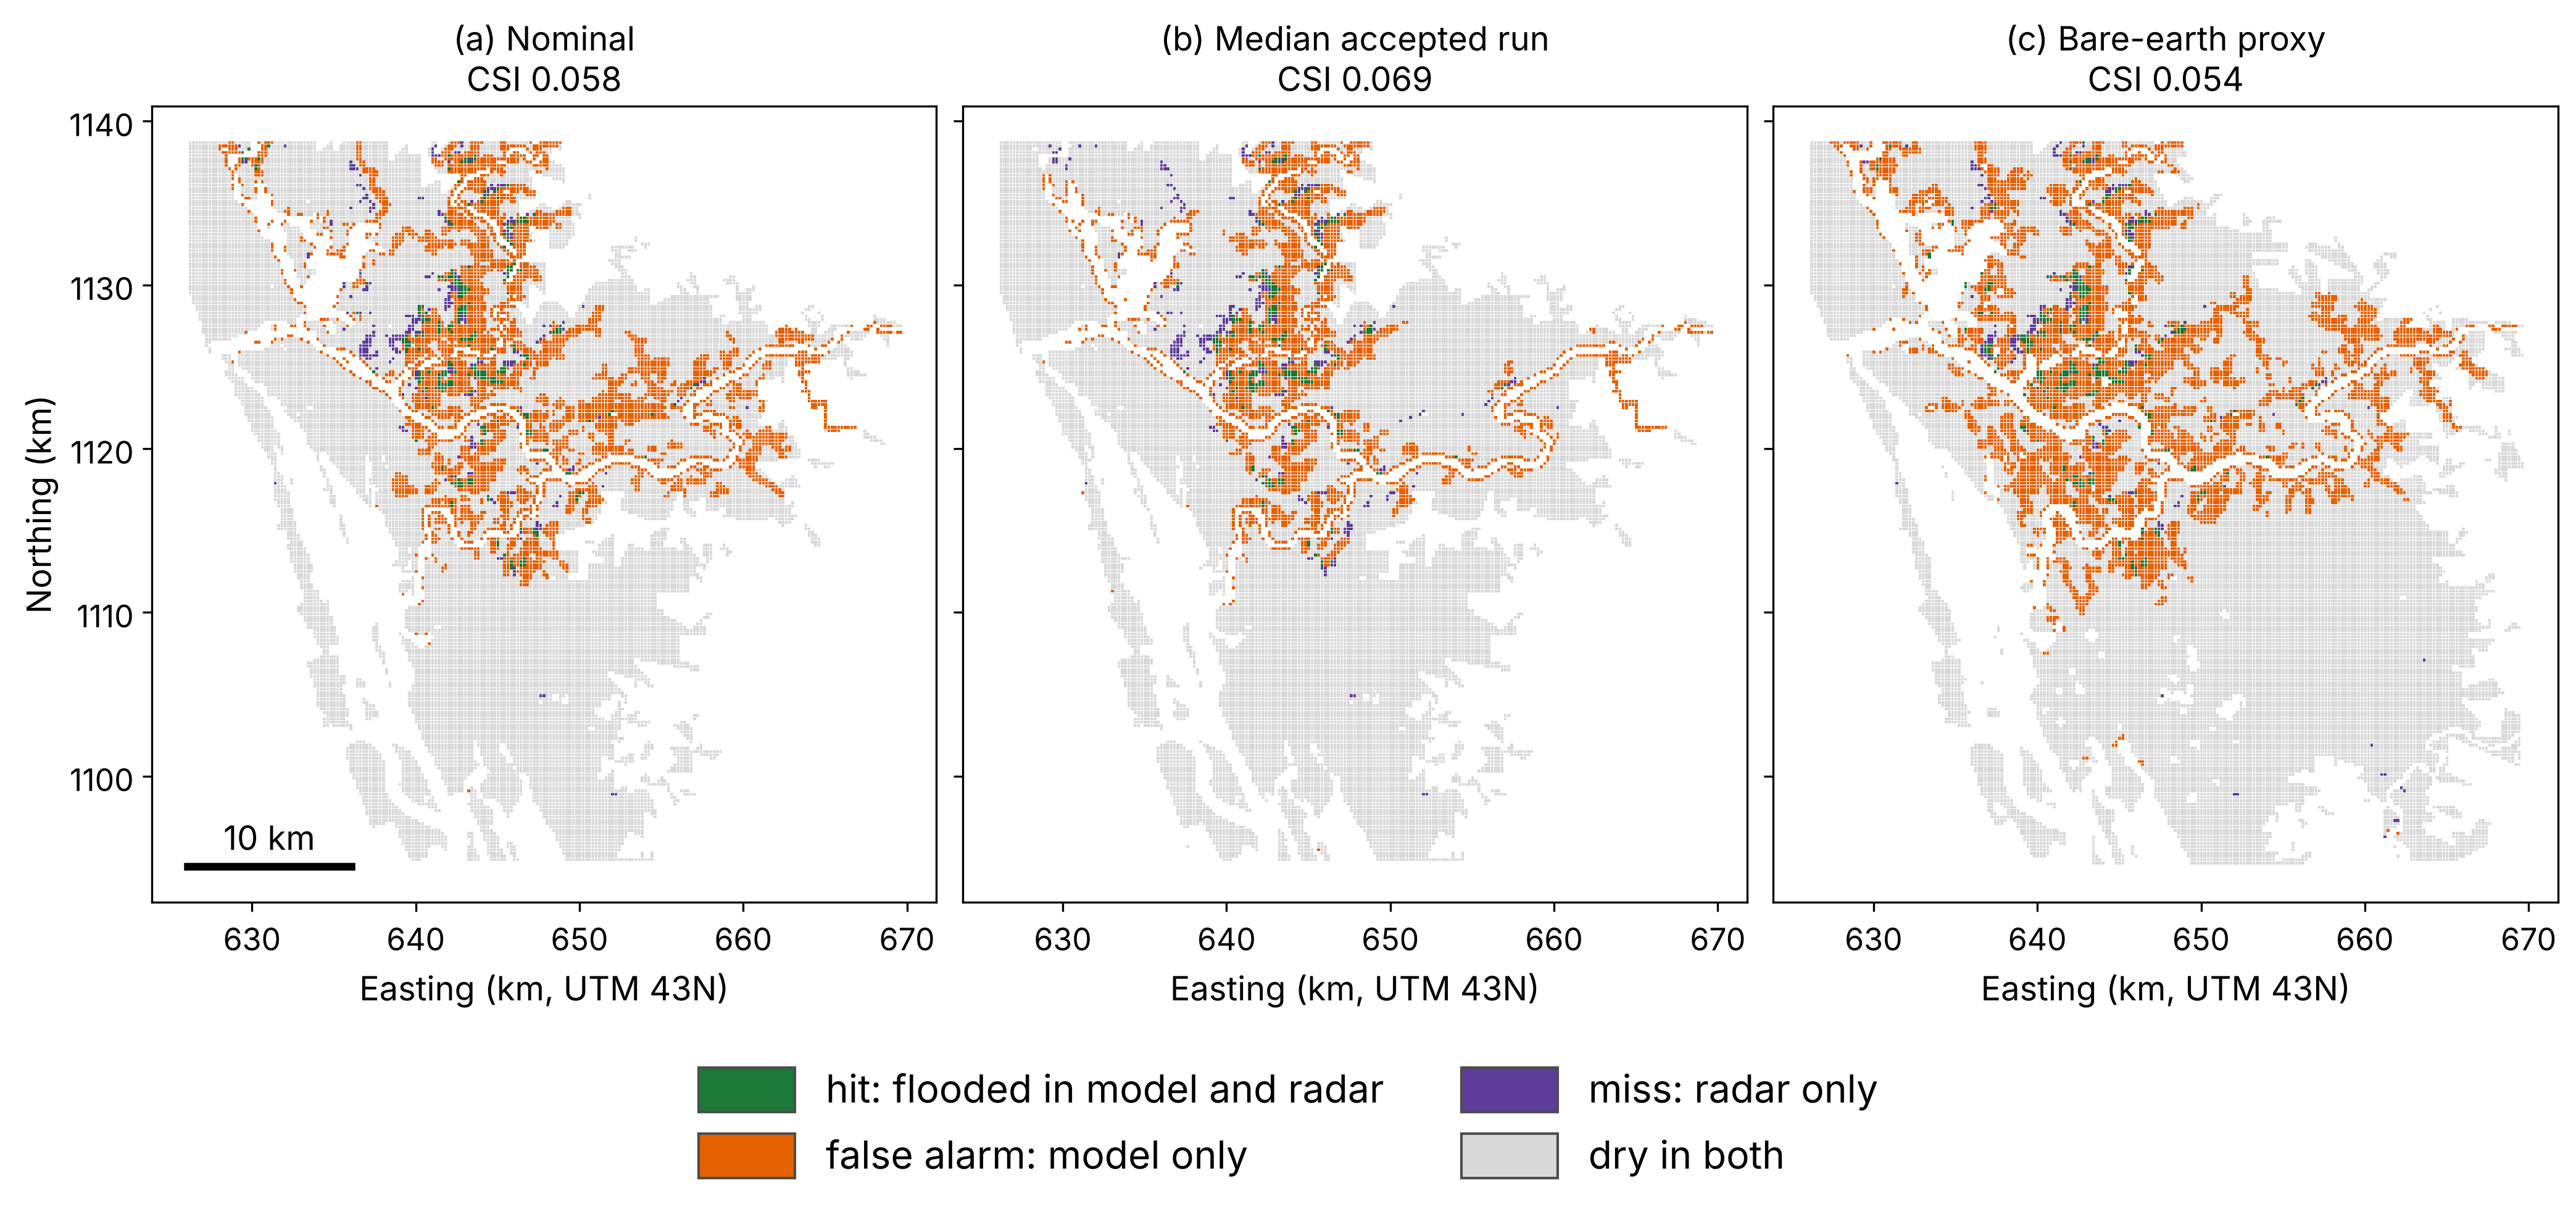
\includegraphics[width=\textwidth]{figures/fig5.png}
\caption{(a) Empirical distribution of peak flooded land for all 600 runs and for the runs passing the HFL test, the radar test and both. (b) Narrowing of the peak flooded-land range, and the number of accepted runs, for other HFL tolerances and open-land hit rates. (c) HFL residuals of all runs (grey) and the accepted runs (blue); the shaded band is the $\pm$0.5~m tolerance.}
\label{fig:uncertainty}
\end{figure}

The accepted runs still span channel depths of 2.1--7.8~m and floodplain roughness multipliers of 0.60--1.49, but depth and roughness compensate each other (correlation 0.70 across the 23 runs, against 0.01 in the prior; Fig.~\ref{fig:conditioning}b): shallow channels pass the HFL only with smooth floodplains. Canopy factors are 0.36--0.90 (median 0.78) and rating errors 0.86--1.11 (median 0.94). The earlier v3 conditioning, with an area cap at three times the radar's, is superseded: on v4 and v5 no run met that cap, because every run of v5 still floods 77~\kmsq{} or more at the radar pass.

\begin{figure}[htbp]
\centering
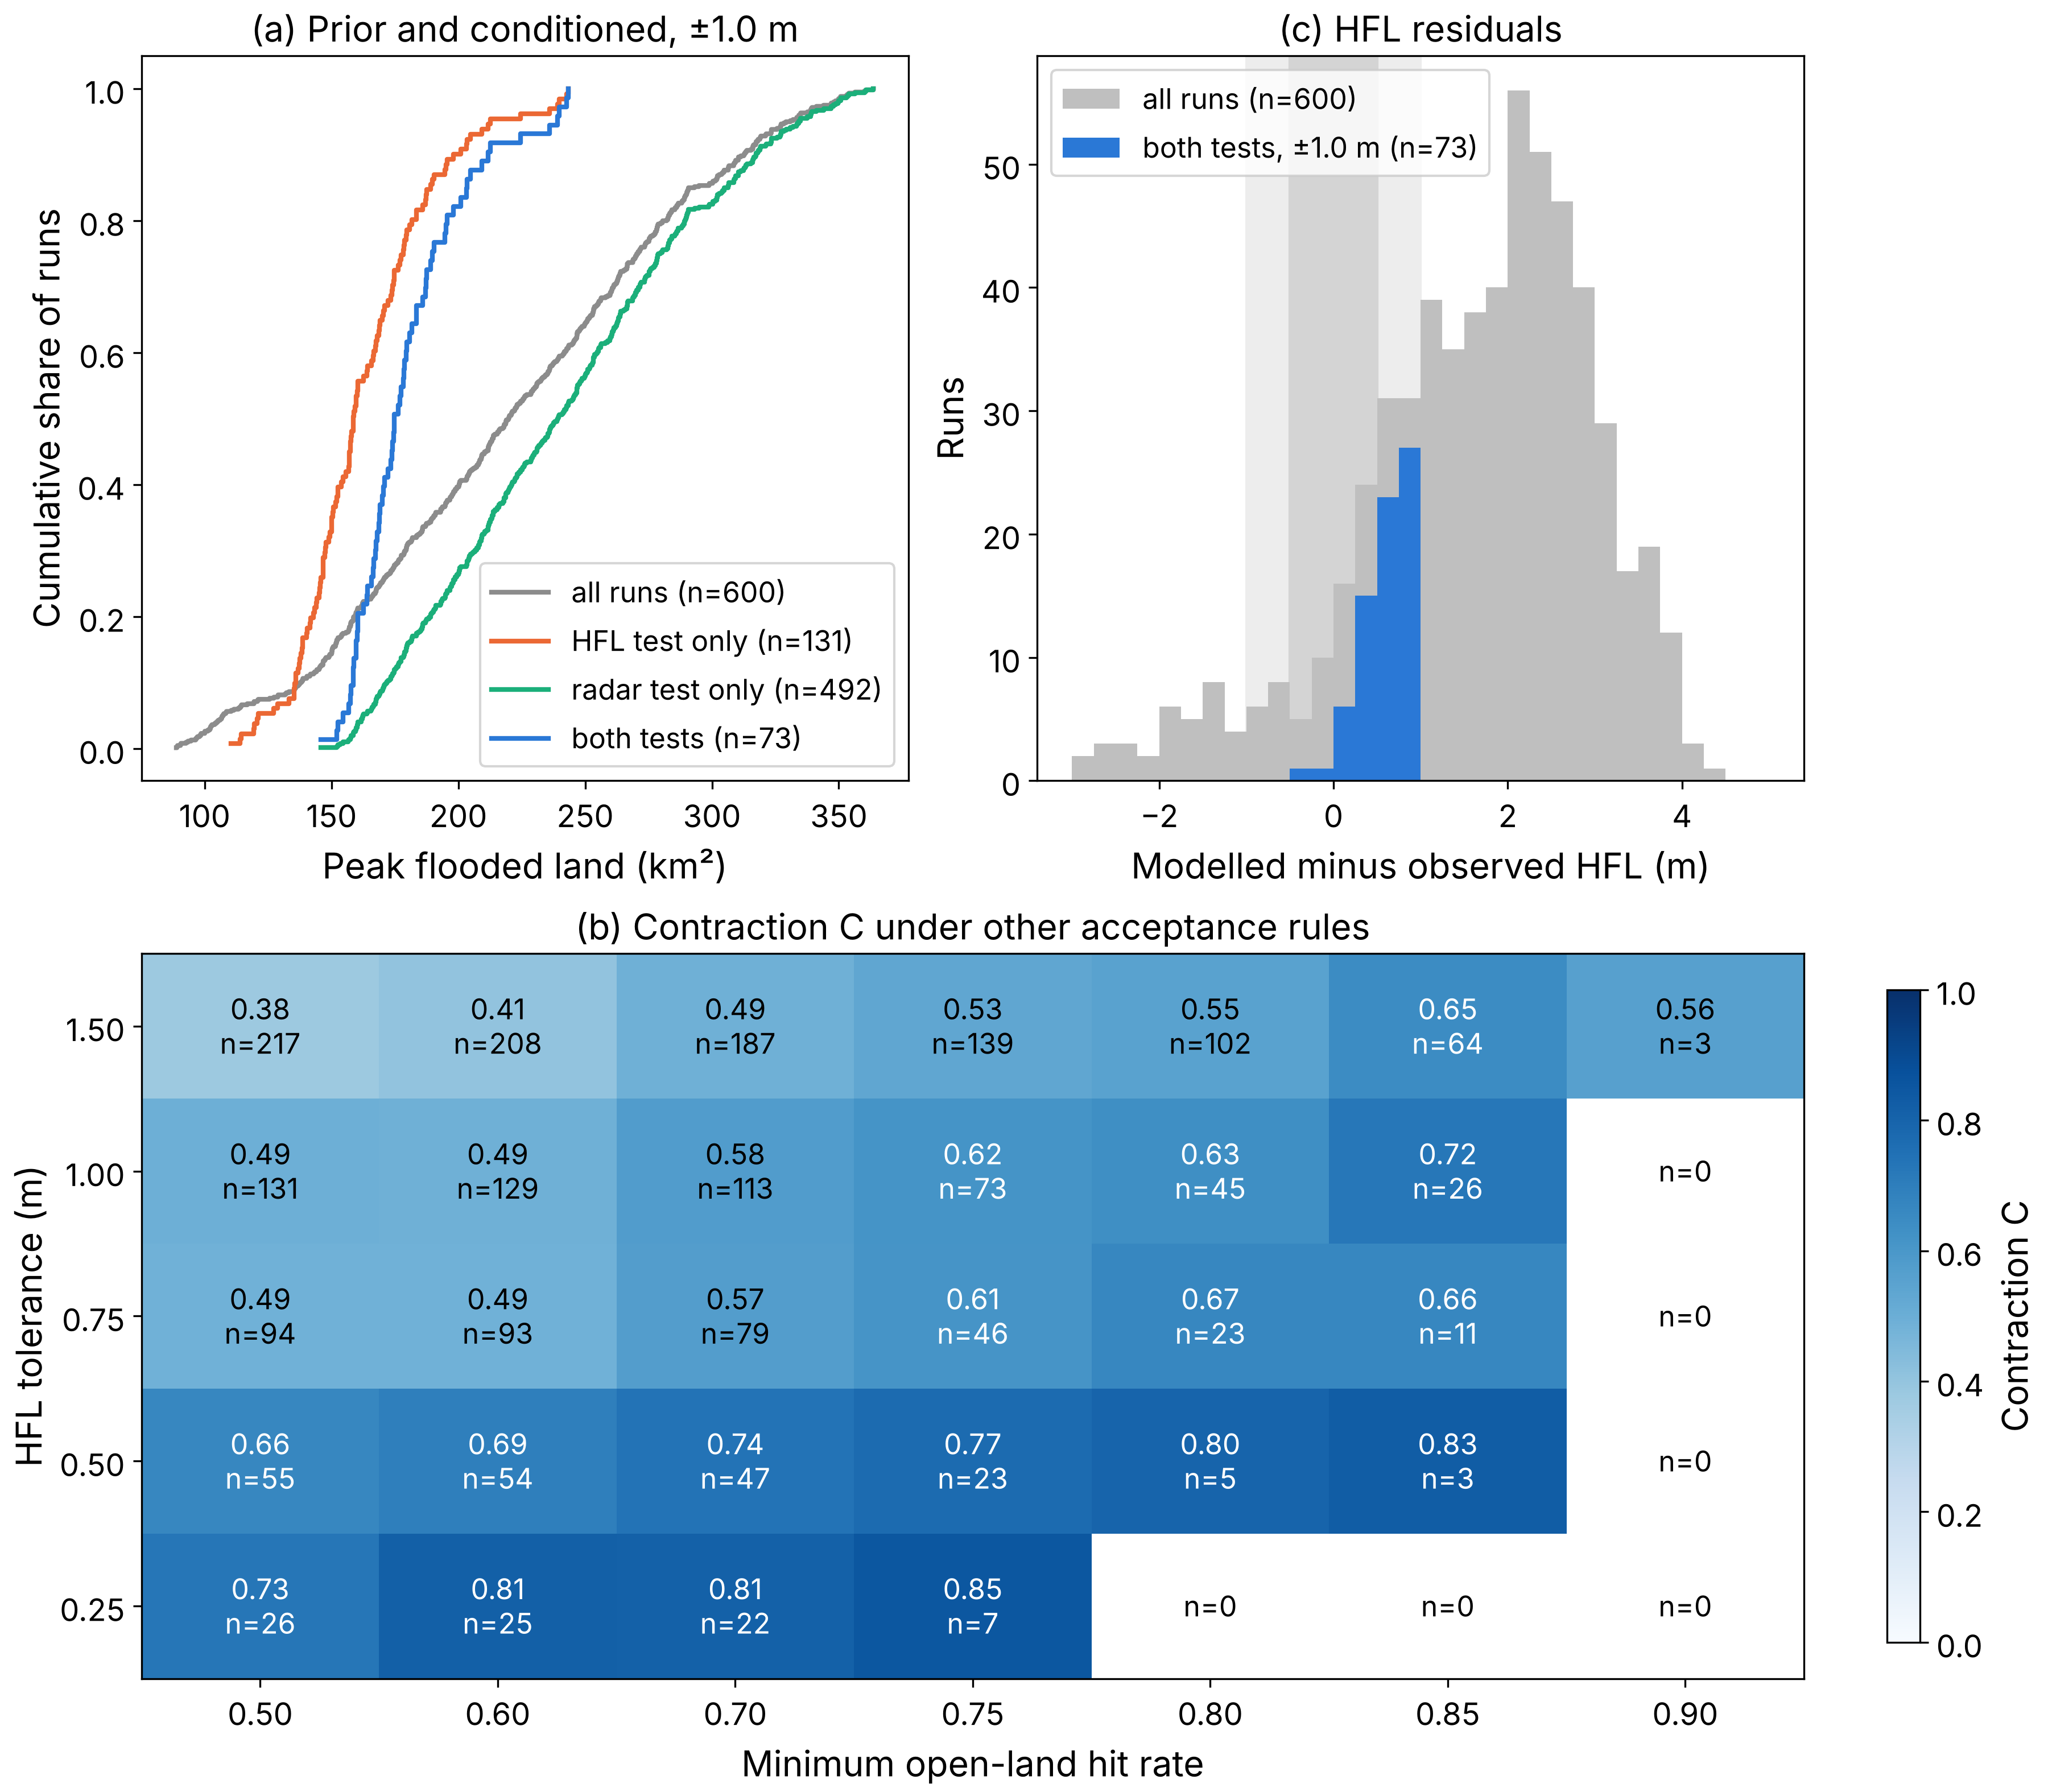
\includegraphics[width=\textwidth]{figures/fig2.png}
\caption{(a) Peak flooded land across the 600-run v5 ensemble (grey) and the 23 runs that pass both the HFL and the radar test (blue). (b) Channel depth against floodplain roughness multiplier for all runs and the accepted runs.}
\label{fig:conditioning}
\end{figure}

\paragraph{Flooded land through time}
The 7 accepted runs of the first 200 were run again to save flooded land every hour (Fig.~\ref{fig:timeseries}). Their peaks (158--182~\kmsq) match the ensemble values exactly. Four runs, all with channel depths of 6.3--6.9~m, peak on 17 August at 07:00--08:00, about a day after the Neeleswaram peak. The other three (depths 2.9--5.1~m) level off near 100--110~\kmsq{} and then flood a further 50--70~\kmsq{} between 17 and 19 August, after the river has begun to fall; their peaks come on 18--19 August. In every run drainage is slow: by the radar pass, when the Neeleswaram flow had fallen by about three quarters, the runs still flood 112--143~\kmsq, or 72--90\% of their peak.

\begin{figure}[htbp]
\centering
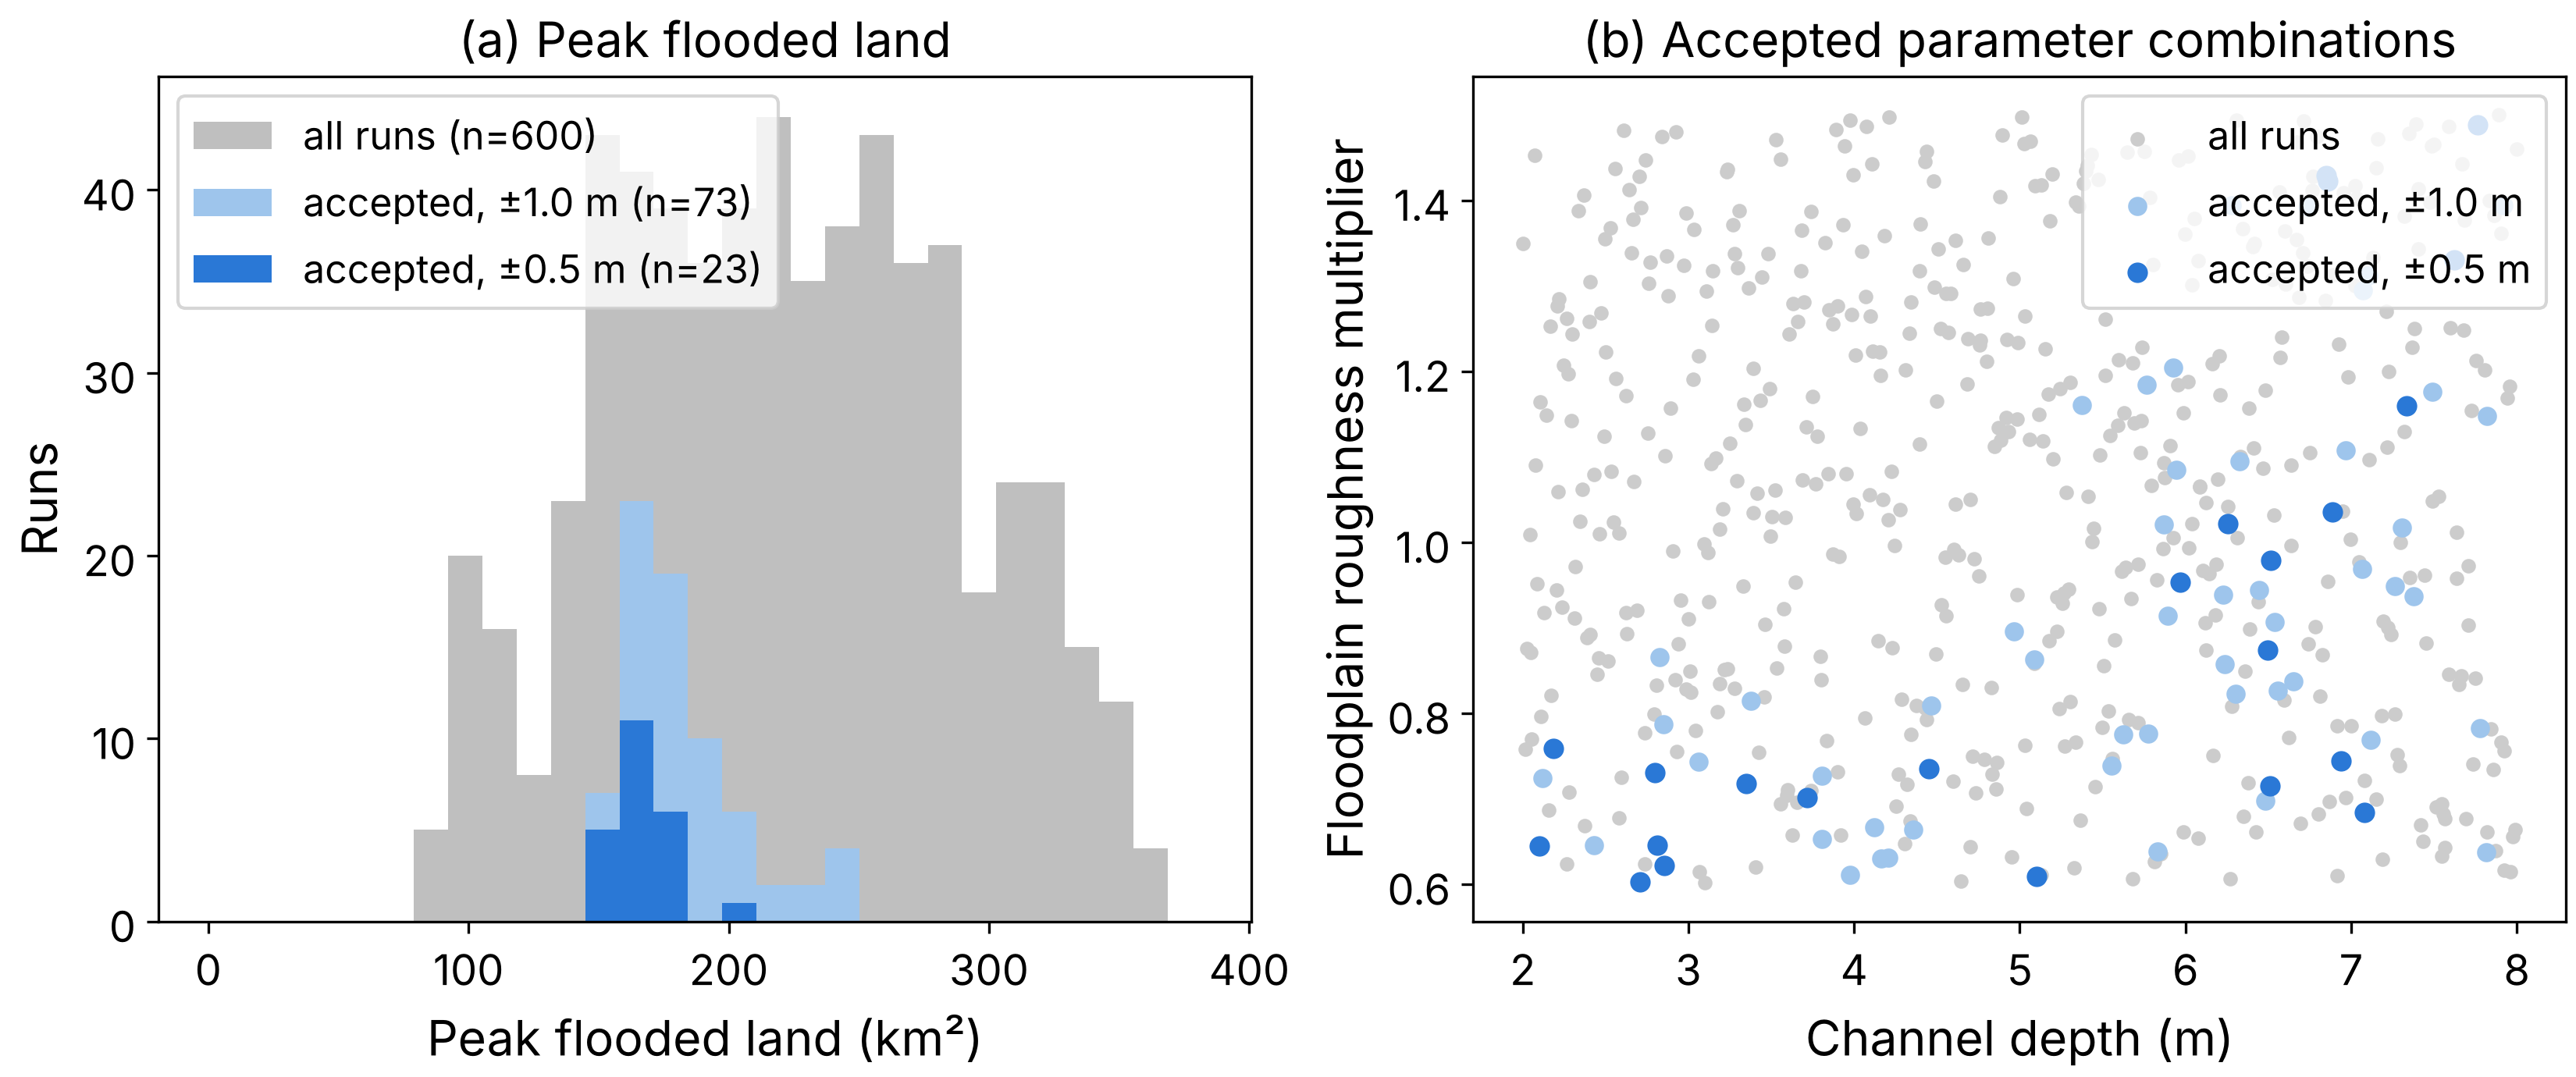
\includegraphics[width=\textwidth]{figures/fig3.png}
\caption{Flooded land (cells dry at the start) through time for the 7 accepted runs of the first 200-run v5 ensemble (blue), with the CWC discharges at Neeleswaram and Arangaly (grey, right axis). The diamond marks the 22~\kmsq{} of open-water flooding on the Sentinel-1 image of 21 August 06:10 IST, a lower bound because radar misses water under trees and in built-up land.}
\label{fig:timeseries}
\end{figure}

\subsection{Agreement with the radar map}
\label{sec:radar}
Passing the radar test does not mean the model reproduces the flood pattern. Table~\ref{tab:confusion} gives the full contingency table for the nominal run and the 7 re-run accepted runs. On all land the accepted runs catch 42--46\% of the radar-flooded cells but nine out of ten of their own flooded cells are not flooded on the radar (false-alarm ratio 0.92--0.93), giving a CSI of 0.067--0.075 and a frequency bias of 5--6. On open land, where C-band radar should see standing water, the hit rate is 0.76--0.86 but the bias is still 7.6--8.8. All 23 accepted runs have an all-land CSI of 0.066--0.075 and an open-land CSI of 0.091--0.098, and no run of the 600 exceeds 0.081 on all land. Model-only flooding covers the whole lower floodplain, not only the tree-covered land (Fig.~\ref{fig:confusion}). Against the radar maps made with other thresholds (18--26~\kmsq{} of open-water flooding) and with a fraction cut-off of 0.3, the all-land CSI of the accepted runs stays between 0.048 and 0.12, so the low skill is not an artefact of the radar classification. We read it as a limitation of the model.

\begin{table}[htbp]
\centering
\caption{Contingency table against the Sentinel-1 map at the radar pass (200~m cells, fraction cut-off 0.5). Accepted runs: range over the 7 re-run accepted runs.}
\label{tab:confusion}
\footnotesize
\resizebox{\textwidth}{!}{%
\begin{tabular}{@{}llrrrrrrrr@{}}
\toprule
Run & Domain & Hits & Misses & False al. & Corr. neg. & Hit rate & FAR & CSI & Bias \\
\midrule
Nominal & all land & 278 & 272 & 4,216 & 17,122 & 0.51 & 0.94 & 0.058 & 8.2 \\
Nominal & open land & 85 & 10 & 993 & 872 & 0.89 & 0.92 & 0.078 & 11.3 \\
Accepted & all land & 228--246 & 295--316 & 2,517--3,048 & 17,800--18,589 & 0.42--0.46 & 0.92--0.93 & 0.067--0.075 & 5.1--6.0 \\
Accepted & open land & 72--82 & 13--23 & 647--756 & 1,094--1,195 & 0.76--0.86 & 0.90--0.91 & 0.093--0.098 & 7.6--8.8 \\
Bare-earth proxy & all land & 340 & 200 & 5,789 & 21,407 & 0.63 & 0.94 & 0.054 & 11.3 \\
\bottomrule
\end{tabular}}
\end{table}

\begin{figure}[htbp]
\centering
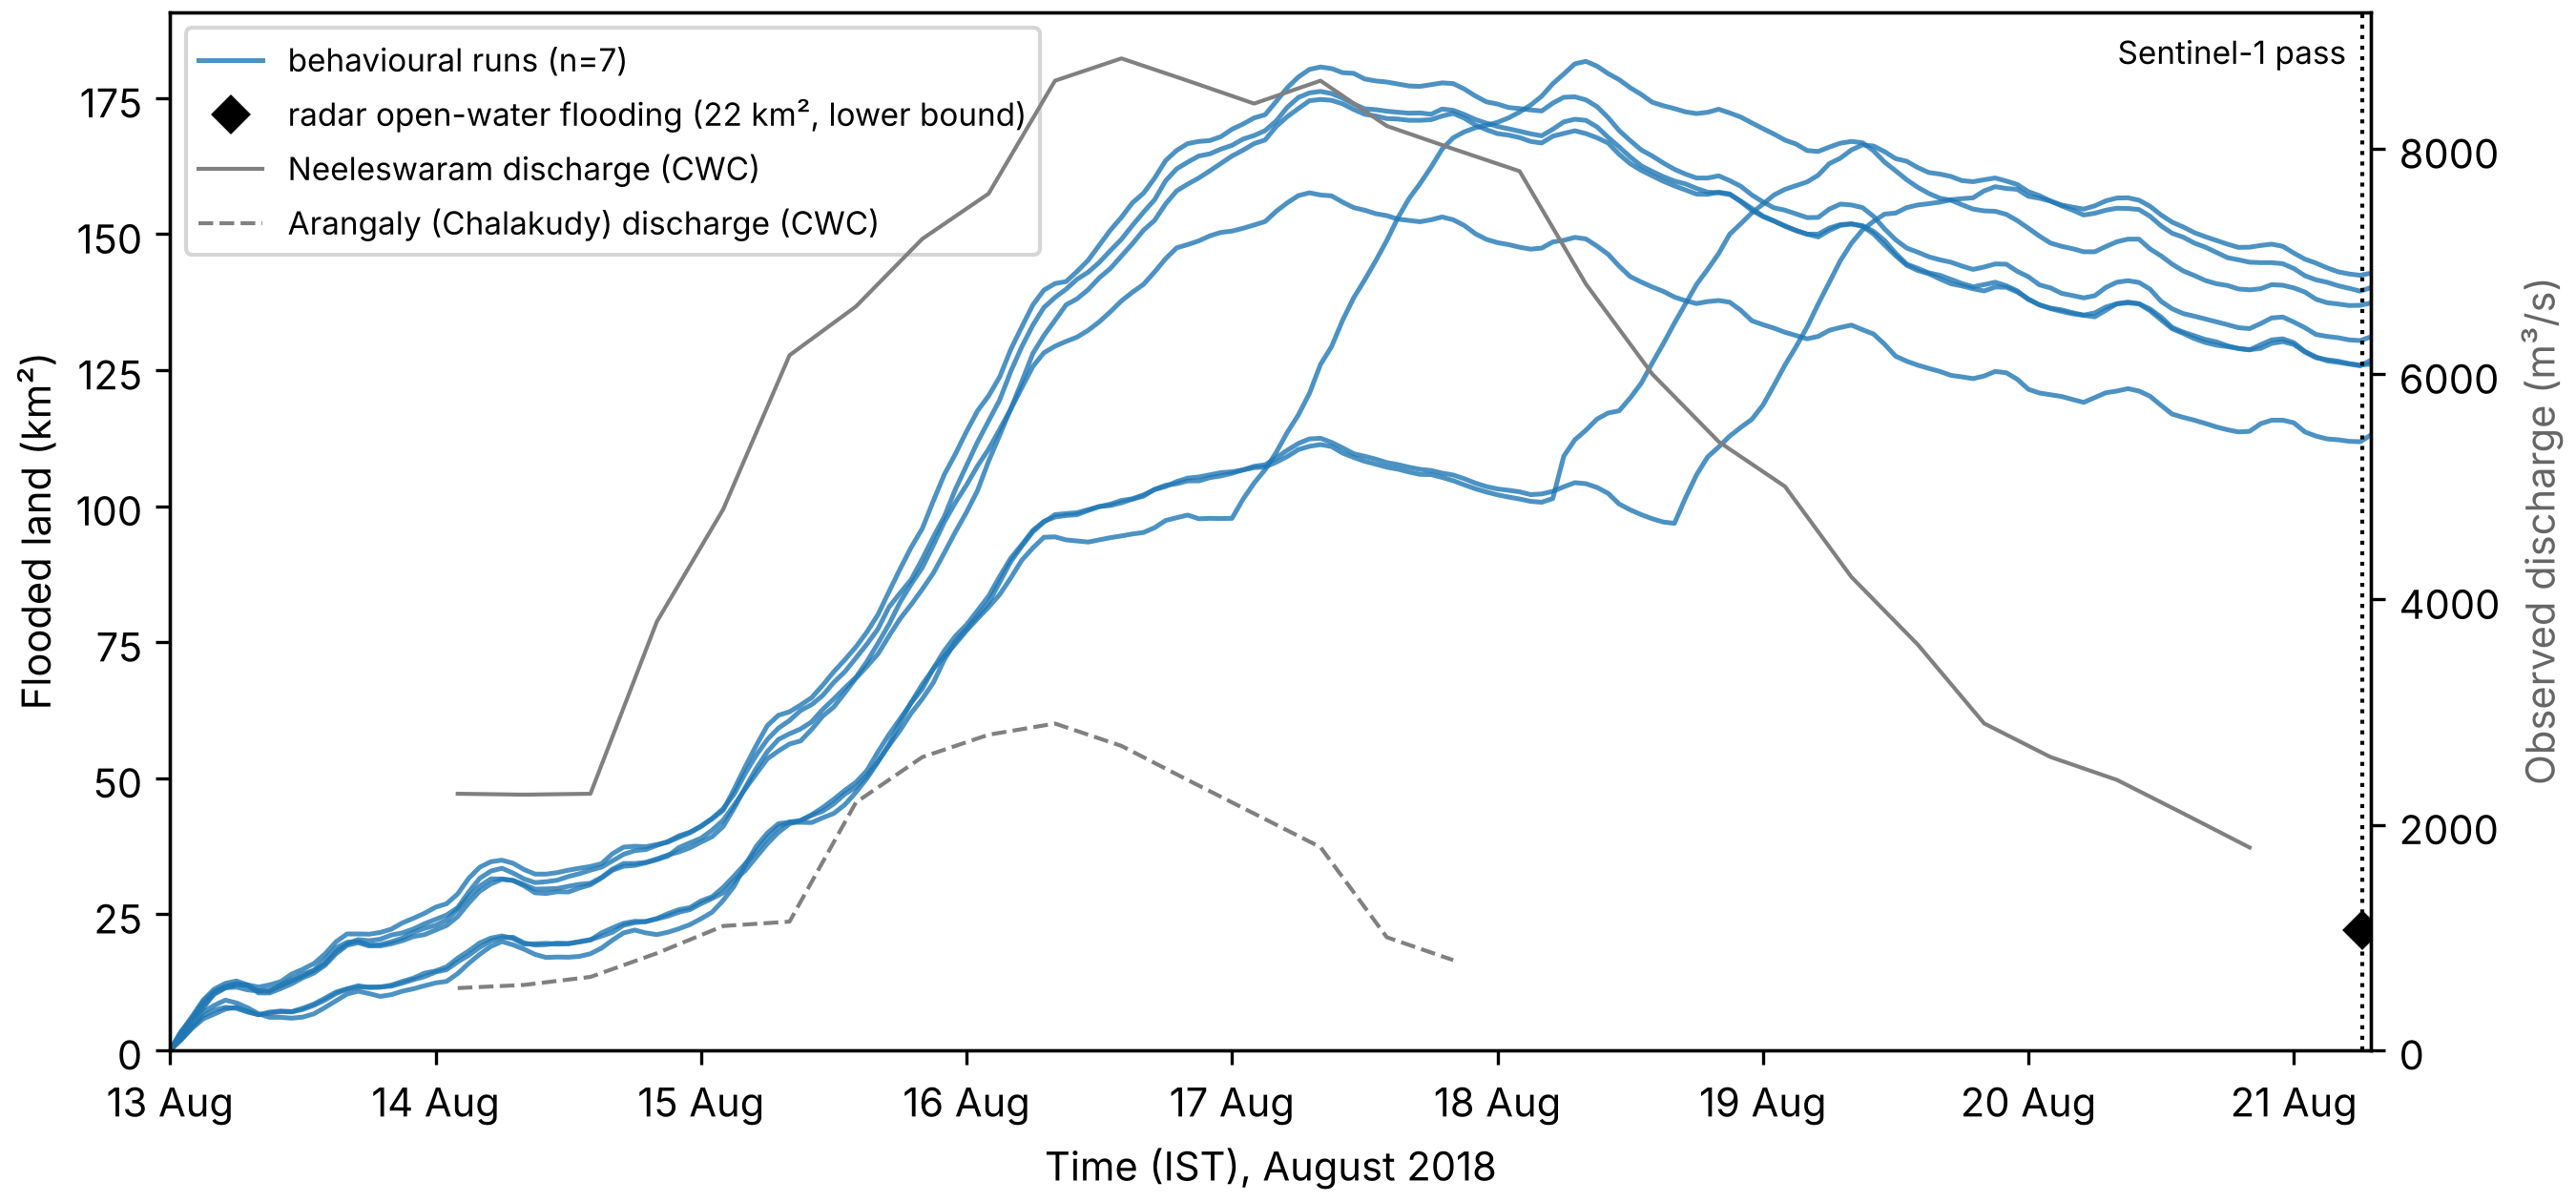
\includegraphics[width=\textwidth]{figures/fig4.png}
\caption{Model against radar at the radar pass, cell by cell, for the nominal run, an accepted run and the bare-earth proxy: flooded in both, in the model only, in the radar only, and dry in both.}
\label{fig:confusion}
\end{figure}

\subsection{Structural tests}
\label{sec:structural}
No structural variant brings the land flooded at the radar pass near the radar's 22~\kmsq{} or raises CSI above 0.085 (Table~\ref{tab:structural}). The bare-earth proxy cuts the HFL error from +2.4~m to $-0.8$~m but floods more land at the pass and does not raise CSI. Full canopy removal and a wider channel mask each lower the HFL error by 0.6--1.1~m. On the 100~m grid (131,654 cells) peak flooded land and the land flooded at the pass are within 1\% of the 200~m run, but the gauge level is 0.9~m higher and the peak comes 12~h later; the area results are thus robust to the grid, while the gauge level is not. On the 400~m grid the inflow boundary did not connect properly to the mesh (boundary inflow fell from 6.9 to $4.5\times10^9$~m\textsuperscript{3}), so it is reported as a failed configuration. A 1.5$\times$ tide or a half-period shift changes flooded land by less than 1\% and the gauge level by less than 0.01~m.

\begin{table}[htbp]
\centering
\caption{Structural variants at nominal parameter values.}
\label{tab:structural}
\small
\resizebox{\textwidth}{!}{%
\begin{tabular}{@{}lrrrrr@{}}
\toprule
Variant & Peak land & Land at pass & Peak volume & HFL error & CSI \\
 & (\kmsq) & (\kmsq) & (\Mcm) & (m) & (all / open) \\
\midrule
Nominal (200 m) & 263 & 180 & 855 & +2.44 & 0.058 / 0.078 \\
Bare-earth proxy & 353 & 245 & 934 & $-0.76$ & 0.054 / 0.076 \\
Full canopy removal & 292 & 201 & 860 & +1.31 & 0.053 / 0.076 \\
Wider channel mask & 210 & 140 & 643 & +1.84 & 0.054 / 0.085 \\
100 m grid & 263 & 179 & 921 & +3.32 & 0.053 / 0.069 \\
Tide $\times$1.5 & 265 & 180 & 856 & +2.44 & 0.058 / 0.078 \\
Tide shifted 6.21 h & 264 & 182 & 854 & +2.44 & 0.058 / 0.078 \\
400 m grid & \multicolumn{5}{c}{failed: inflow not connected to the mesh} \\
\bottomrule
\end{tabular}}
\end{table}

\section{Discussion}
\label{sec:discussion}

\paragraph{What the observations can and cannot do}
The two observations did two different jobs. They exposed structural errors that the GSA could not, and the HFL then narrowed the spread of the predicted flood area by about three quarters within the ensemble. They did not make the model spatially right: the accepted runs reproduce most of the open-land flooding the radar sees, but flood five to six times too much land at the radar pass. The narrowing is therefore a statement about parameter uncertainty given this model structure, not about predictive accuracy. The v1 screening ranked the right factors on a model that was 10~m wrong, which is a warning for GSA studies without validation.

\paragraph{Structural discrepancy}
The ensemble excludes several sources of error: terrain error beyond the canopy factor (buildings, embankments, DSM noise), channel geometry beyond a uniform depth below the cell minimum, grid resolution, local rainfall and lateral inflows, and embankments and drainage structures. The structural tests show that none of the single changes we could make removes the excess flooding after the peak, and that the gauge level shifts by 0.9~m between grids, more than the 0.5~m acceptance tolerance. A structural error term of that size (the 1~m tolerance or $s$ = 1~m weighting in Table~\ref{tab:robust}) roughly halves the narrowing, to 35--72\%. We consider these the honest bounds on what one HFL mark achieves here. The late rise in some runs (Fig.~\ref{fig:timeseries}) may come from water crossing an embankment-like ridge in the DSM; this is a hypothesis we have not tested.

\paragraph{Channel geometry dominates}
Channel depth leads peak area, volume and the gauge level on both model versions. The lack of bathymetry is therefore the largest single uncertainty, which argues for cheap channel surveys or satellite-derived depth.

\paragraph{Canopy correction}
The canopy factor ranks fourth for peak area, and full canopy removal lowers the HFL error by 1.1~m. The accepted runs favour removing most of the canopy height (median factor 0.78) but do not exclude 0.36. Because the range of this factor is exploratory, we read this as a preference rather than an estimate. DSM-based models of vegetated tropical floodplains should treat the correction as an explicit uncertain factor, or test a bare-earth product such as FABDEM \citep{hawker2022}.

\paragraph{Equifinality}
Channel depth and floodplain roughness compensate each other (correlation 0.70 in the 23 accepted runs), so one HFL mark cannot separate them, in line with the equifinality that motivates GLUE \citep{beven1992}. A second gauge or an image taken near the peak could.

\paragraph{Radar limits}
Over 80\% of land cells are tree cover, where C-band radar sees little open water, and the only scene was taken 5 days after the peak. These limits explain why the radar can serve only as a lower bound with a hit-rate test \citep[rather than as a binary pattern to match;][]{aronica2002}. They do not explain the false alarms on open land, which point to the slow drainage of the model.

\paragraph{What transfers}
Three findings are likely to hold in other open-data models of forested monsoon floodplains: that a single high-flood mark constrains the predicted area mainly through channel depth and floodplain roughness and leaves them in compensation; that a post-peak radar scene over tree cover can reject the driest runs but not the wettest; and that the narrowing depends on the acceptance tolerance and on any structural error term at least as much as on the observation itself. The ranking of factors, the size of the narrowing, the negligible role of sea level and the slow drainage are specific to the Periyar model and the 2018 event.

\subsection{Limitations}
\begin{itemize}
\item Slow drainage. At the radar pass every run still floods 77--250~\kmsq{} of land against 22~\kmsq{} of open water on the radar, and no structural variant we tested removes this.
\item The tide is synthetic, and there is no local rainfall or lateral inflow on the model domain. Rainfall would add water and so would not cure the excess flooding; its effect on timing we cannot quantify with the data available. The tide tests and the Morris screening show a negligible effect of sea level, for these tests and this model only.
\item Boundary flows were digitised from report figures, and the gauge location was inferred from the water mask; the HFL datum is assumed equal to the DEM datum.
\item The model uses 200~m cells and one event; the bare-earth test uses a proxy, not FABDEM.
\item Factor ranges are expert assumptions, sampled independently; the channel depth and canopy ranges are exploratory, and three factors were fixed in the conditioning ensemble (11\% of the summed $\mu^*$ for area).
\end{itemize}

\section{Conclusions}
\label{sec:conclusions}

An open-data D-Flow FM model of the 2018 Periyar flood, built with HYDROLIB-core, was screened with 180 Morris runs and conditioned with a 600-run Latin hypercube. Validation against one high-flood level and one Sentinel-1 scene exposed three structural errors and one missing tributary that the sensitivity analysis did not. On the final model, channel depth, floodplain roughness and rating-curve error dominate the flooded area, as they did before the last revision, and sea level is negligible. Conditioning on the same two observations narrowed the peak flooded-area range within the ensemble by about 77\% (76--88\% under resampling, 49--72\% with a 1~m tolerance for structural error), to 146--198~\kmsq; the HFL mark does most of this, and channel depth and floodplain roughness stay in compensation. The narrowing is conditional on the model structure. The accepted runs still flood far more land than the radar shows after the peak, and none of the structural changes tested removes that excess; channel bathymetry, bare-earth terrain and a second observation time are the most direct ways to address it.

\section*{Code and data availability}
All scripts (model build, sensitivity runs, radar flood map, validation, structural tests, analysis and figures), the digitised CWC flow records, the radar maps and the per-run results of every ensemble are in the HYDROLIB-core fork at \url{https://github.com/karthice1/HYDROLIB-core}, under \texttt{research/periyar} and \texttt{research/gsa}; \texttt{research/periyar/README.md} lists the software versions and the command behind every table and figure. [Zenodo DOI of the archived release to be inserted.]

\section*{CRediT authorship contribution statement}
\textbf{Karthik V:} [to be completed by the authors]. \textbf{Roopa D:} [to be completed by the authors].

\section*{Declaration of competing interest}
[To be completed by the authors.]

\section*{Acknowledgements}
[To be completed by the authors.]

\begin{thebibliography}{99}
\expandafter\ifx\csname natexlab\endcsname\relax\def\natexlab#1{#1}\fi

\bibitem[{Aronica et~al.(2002)Aronica, Bates and Horritt}]{aronica2002}
Aronica, G.T., Bates, P.D., Horritt, M.S., 2002. Assessing the uncertainty in distributed model predictions using observed binary pattern information within {GLUE}. Hydrological Processes 16, 2001--2016.

\bibitem[{Bates et~al.(2004)Bates, Horritt, Aronica and Beven}]{bates2004}
Bates, P.D., Horritt, M.S., Aronica, G., Beven, K.J., 2004. Bayesian updating of flood inundation likelihoods conditioned on flood extent data. Hydrological Processes 18, 3347--3370.

\bibitem[{Beven and Binley(1992)}]{beven1992}
Beven, K., Binley, A., 1992. The future of distributed models: model calibration and uncertainty prediction. Hydrological Processes 6, 279--298. \url{https://doi.org/10.1002/hyp.3360060305}.

\bibitem[{Campolongo et~al.(2007)Campolongo, Cariboni and Saltelli}]{campolongo2007}
Campolongo, F., Cariboni, J., Saltelli, A., 2007. An effective screening design for sensitivity analysis of large models. Environmental Modelling \& Software 22, 1509--1518. \url{https://doi.org/10.1016/j.envsoft.2006.10.004}.

\bibitem[{CWC(2018)}]{cwc2018}
CWC (Central Water Commission), 2018. Study Report: Kerala Floods of August 2018. Hydrological Studies Organisation, Hydrology (S) Directorate, Government of India, New Delhi.

\bibitem[{ESA(2021)}]{esa2021}
ESA, 2021. Copernicus DEM GLO-30 (Copernicus Digital Elevation Model, 30 m). European Space Agency. \url{https://doi.org/10.5270/ESA-c5d3d65}. \textcopyright{} DLR e.V. 2010--2014 and \textcopyright{} Airbus Defence and Space GmbH 2014--2018, provided under COPERNICUS by the European Union and ESA.

\bibitem[{Government of Kerala and UN(2018)}]{pdna2018}
Government of Kerala and UN, 2018. Kerala Post Disaster Needs Assessment: Floods and Landslides, August 2018. Government of Kerala with the United Nations (UNDP), Thiruvananthapuram.

\bibitem[{Hall et~al.(2005)Hall, Tarantola, Bates and Horritt}]{hall2005}
Hall, J.W., Tarantola, S., Bates, P.D., Horritt, M.S., 2005. Distributed sensitivity analysis of flood inundation model calibration. Journal of Hydraulic Engineering 131, 117--126. \url{https://doi.org/10.1061/(ASCE)0733-9429(2005)131:2(117)}.

\bibitem[{Hawker et~al.(2022)Hawker, Uhe, Paulo, Sosa, Savage, Sampson and Neal}]{hawker2022}
Hawker, L., Uhe, P., Paulo, L., Sosa, J., Savage, J., Sampson, C., Neal, J., 2022. A 30 m global map of elevation with forests and buildings removed. Environmental Research Letters 17, 024016. \url{https://doi.org/10.1088/1748-9326/ac4d4f}.

\bibitem[{Herman and Usher(2017)}]{herman2017}
Herman, J., Usher, W., 2017. {SALib}: An open-source Python library for sensitivity analysis. Journal of Open Source Software 2, 97. \url{https://doi.org/10.21105/joss.00097}.

\bibitem[{Kernkamp et~al.(2011)Kernkamp, Van~Dam, Stelling and de~Goede}]{kernkamp2011}
Kernkamp, H.W.J., Van Dam, A., Stelling, G.S., de Goede, E.D., 2011. Efficient scheme for the shallow water equations on unstructured grids with application to the Continental Shelf. Ocean Dynamics 61, 1175--1188. \url{https://doi.org/10.1007/s10236-011-0423-6}.

\bibitem[{Mishra and Shah(2018)}]{mishra2018}
Mishra, V., Shah, H.L., 2018. Hydroclimatological perspective of the Kerala flood of 2018. Journal of the Geological Society of India 92, 645--650. \url{https://doi.org/10.1007/s12594-018-1079-3}.

\bibitem[{Montanari et~al.(2009)Montanari, Hostache, Matgen, Schumann, Pfister and Hoffmann}]{montanari2009}
Montanari, M., Hostache, R., Matgen, P., Schumann, G., Pfister, L., Hoffmann, L., 2009. Calibration and sequential updating of a coupled hydrologic-hydraulic model using remote sensing-derived water stages. Hydrology and Earth System Sciences 13, 367--380. \url{https://doi.org/10.5194/hess-13-367-2009}.

\bibitem[{Morris(1991)}]{morris1991}
Morris, M.D., 1991. Factorial sampling plans for preliminary computational experiments. Technometrics 33, 161--174.

\bibitem[{Pappenberger et~al.(2005)Pappenberger, Beven, Hunter, Bates, Gouweleeuw, Thielen and de~Roo}]{pappenberger2005}
Pappenberger, F., Beven, K.J., Hunter, N.M., Bates, P.D., Gouweleeuw, B.T., Thielen, J., de Roo, A.P.J., 2005. Cascading model uncertainty from medium range weather forecasts (10 days) through a rainfall-runoff model to flood inundation predictions within the European Flood Forecasting System ({EFFS}). Hydrology and Earth System Sciences 9, 381--393. \url{https://doi.org/10.5194/hess-9-381-2005}.

\bibitem[{Pekel et~al.(2016)Pekel, Cottam, Gorelick and Belward}]{pekel2016}
Pekel, J.F., Cottam, A., Gorelick, N., Belward, A.S., 2016. High-resolution mapping of global surface water and its long-term changes. Nature 540, 418--422. \url{https://doi.org/10.1038/nature20584}.

\bibitem[{Pianosi et~al.(2016)Pianosi, Beven, Freer, Hall, Rougier, Stephenson and Wagener}]{pianosi2016}
Pianosi, F., Beven, K., Freer, J., Hall, J.W., Rougier, J., Stephenson, D.B., Wagener, T., 2016. Sensitivity analysis of environmental models: A systematic review with practical workflow. Environmental Modelling \& Software 79, 214--232. \url{https://doi.org/10.1016/j.envsoft.2016.02.008}.

\bibitem[{Saltelli et~al.(2008)Saltelli, Ratto, Andres, Campolongo, Cariboni, Gatelli, Saisana and Tarantola}]{saltelli2008}
Saltelli, A., Ratto, M., Andres, T., Campolongo, F., Cariboni, J., Gatelli, D., Saisana, M., Tarantola, S., 2008. Global Sensitivity Analysis: The Primer. John Wiley \& Sons, Chichester.

\bibitem[{Savage et~al.(2016)Savage, Bates, Freer, Neal and Aronica}]{savage2016}
Savage, J.T.S., Bates, P., Freer, J., Neal, J., Aronica, G.T., 2016. When does spatial resolution become spurious in probabilistic flood inundation predictions? Hydrological Processes 30, 2014--2032. \url{https://doi.org/10.1002/hyp.10749}.

\bibitem[{Sudheer et~al.(2019)Sudheer, Bhallamudi, Narasimhan, Thomas, Bindhu, Vema and Kurian}]{sudheer2019}
Sudheer, K.P., Bhallamudi, S.M., Narasimhan, B., Thomas, J., Bindhu, V.M., Vema, V., Kurian, C., 2019. Role of dams on the floods of August 2018 in Periyar River Basin, Kerala. Current Science 116, 780--794. \url{https://doi.org/10.18520/cs/v116/i5/780-794}.

\bibitem[{Teng et~al.(2017)Teng, Jakeman, Vaze, Croke, Dutta and Kim}]{teng2017}
Teng, J., Jakeman, A.J., Vaze, J., Croke, B.F.W., Dutta, D., Kim, S., 2017. Flood inundation modelling: A review of methods, recent advances and uncertainty analysis. Environmental Modelling \& Software 90, 201--216. \url{https://doi.org/10.1016/j.envsoft.2017.01.006}.

\bibitem[{Tolan et~al.(2024)}]{tolan2024}
Tolan, J., Yang, E., Nosarzewski, B., Couairon, G., Vo, H.V., Brandt, J., Spore, J., Majumdar, S., Haziza, D., Vamaraju, J., Moutakanni, T., Bojanowski, P., Johns, T., White, B., Tiecke, T., Couprie, C., Saenz, E., 2024. Very high resolution canopy height maps from {RGB} imagery using self-supervised vision transformer and convolutional decoder trained on aerial lidar. Remote Sensing of Environment 300, 113888. \url{https://doi.org/10.1016/j.rse.2023.113888}.

\bibitem[{Zanaga et~al.(2022)}]{zanaga2022}
Zanaga, D., Van De Kerchove, R., Daems, D., De Keersmaecker, W., Brockmann, C., Kirches, G., Wevers, J., Cartus, O., Santoro, M., Fritz, S., Lesiv, M., Herold, M., Tsendbazar, N.E., Xu, P., Ramoino, F., Arino, O., 2022. {ESA} {WorldCover} 10 m 2021 v200. Zenodo. \url{https://doi.org/10.5281/zenodo.7254221}.

\end{thebibliography}

\end{document}
